\section{Metodologia}
\label{sec:metodologia}

\subsection{Dati e disegno sperimentale}
Indichiamo con $q_t$ la domanda al turno $t$, con $H_{<t}$ la cronologia precedente, con $C_d$ il corpus del dominio $d$ e con $G_t\subseteq C_d$ l'insieme dei passaggi pertinenti per il turno. Nel 2a il sistema riceve $(q_t,H_{<t},C_d)$ e restituisce un ranking di documenti. Il riferimento $G_t$ serve alla supervisione e alla valutazione. Nel 2b gli organizzatori forniscono $G_t$ come parte dell'input: il sistema deve formulare una risposta a partire dal turno, dalla cronologia e dal testo di questi passaggi. La qualità della risposta può così essere studiata a parità di evidenza disponibile \cite{reteco,evaluation}.

Il rilascio pubblico comprende 496 conversazioni di addestramento (2\,113 turni) e 211 conversazioni di sviluppo (858 turni) in undici domini \cite{data}. A partire dal solo \emph{train} ufficiale ricaviamo una validazione interna con seme 42 e quota nominale del 15\% per il 2a e del 10\% per il 2b. L'unità di partizione è la conversazione: tutti i turni dello stesso dialogo appartengono alla stessa partizione. Per il 2a si interroga il corpus completo del dominio in ciascuna partizione. Il \emph{dev} ufficiale è riservato al confronto dopo la selezione della configurazione sulla validazione interna.

\subsection{Profondità ricorrente in inferenza}
Sia $F_j$ uno strato di un decoder di $L$ strati, con indice a partire da zero. L'intervento usa per default lo strato centrale inferiore, $j=\lfloor(L-1)/2\rfloor$. Se $h$ è il tensore in ingresso allo strato, definiamo
\begin{equation}
 h^{(0)}=h,\qquad
 h^{(r+1)}=F_j\bigl(h^{(r)};M,P\bigr),
 \qquad r=0,\ldots,R-1,
 \label{eq:metodo-ricorrenza}
\end{equation}
dove $M$ è la maschera di attenzione e $P$ raccoglie le informazioni posizionali. Ogni applicazione riceve lo stato prodotto dalla precedente sulla stessa sequenza tokenizzata, con la stessa maschera e le stesse posizioni. Gli strati a valle ricevono $h^{(R)}$. Con $R=1$ si esegue il normale percorso del decoder. Con $R=2$ si applica $F_j$ una volta in più. Si ottengono $L+R-1$ applicazioni di strato per \emph{forward}, condividendo tutti i pesi dello strato ripetuto.

L'implementazione riutilizza il modulo del modello preaddestrato in modalità di valutazione. Se il checkpoint include un adattatore, il confronto di profondità usa lo stesso adattatore in ogni condizione. Disattiviamo la cache chiave--valore in tutti i bracci di questo confronto, incluso il controllo $R=1$. Nel riordinatore un \emph{forward} produce il punteggio di una coppia o di un batch di coppie. Nel generatore la ricorrenza si applica a ogni \emph{forward} della decodifica, e con cache disabilitata il modello rielabora il prefisso a ogni passo. Il numero di applicazioni di strato descrive quindi l'intervento per \emph{forward}, mentre la latenza va misurata a livello di query o di risposta.

\subsection{Subtrack 2a. Dal corpus al ranking}
\paragraph{Rappresentazione della domanda e candidati.}
La Figura~\ref{fig:metodo-2a} mostra il passaggio dal recupero sul corpus al confronto tra profondità. Costruiamo una query contestuale a partire da domanda e storia e una riscrittura testuale con Qwen3-4B-Instruct-2507, indicata come \texttt{reasoned} nei log. Le due formulazioni consentono di misurare quanto cambi il recupero a monte quando si esplicita il bisogno informativo. Per il canale lessicale usiamo BM25 nativo di Pyserini/Lucene, con $k_1=0{,}9$ e $b=0{,}4$. Per il canale denso, Qwen3-Embedding-0.6B codifica query e passaggio separatamente \cite{qwen}. Estraiamo lo stato dell'ultimo token valido e normalizziamo i vettori in norma euclidea. Il prodotto scalare tra i vettori normalizzati equivale alla similarità coseno. Il budget è di 512 token per la query e 384 per il documento.

\begin{figure}[htbp]
 \centering
 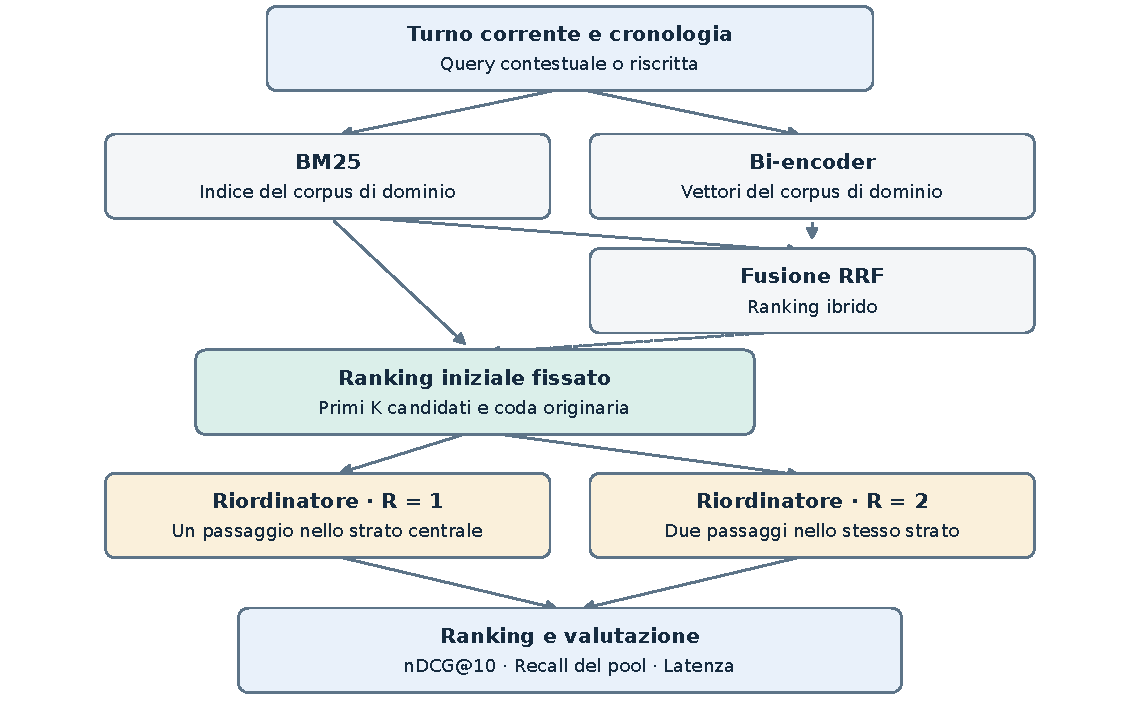
\includegraphics[width=\linewidth]{metodologia_2a.pdf}
 \caption{Flusso del 2a. I canali lessicale e denso producono i ranking del primo stadio. Il confronto principale congela il ranking BM25 contestuale e confronta i riordinatori sui medesimi primi $K$ candidati. La freccia tratteggiata indica l’uso del ranking ibrido come secondo pool, fissato per tutti i bracci del relativo confronto.}
 \label{fig:metodo-2a}
\end{figure}

\paragraph{Adattamento del bi-encoder.}
Adattiamo il bi-encoder con LoRA (rango 16, $\alpha=32$, dropout 0,05) \cite{lora}. Per ogni turno selezioniamo un passaggio positivo tra quelli annotati. Il positivo compete con due negativi difficili campionati da una riserva fino a 40 risultati BM25 e con i positivi associati agli altri esempi del minibatch. La riserva è ricavata dalla query contestuale escludendo i passaggi annotati come pertinenti per quel turno. Nel modo alternato, l'indice dell'esempio e la parità dell'epoca determinano quale formulazione della query si usa. Ogni esempio usa una sola formulazione per epoca e passa all'altra nell'epoca successiva, quando entrambe sono disponibili.

Sia $x_i$ la query effettivamente usata dall'esempio $i$, $p_i$ il suo passaggio positivo e $N_i$ la lista delle posizioni negative. Il contributo dell'esempio alla perdita è
\begin{equation}
 \ell_i=-\log
 \frac{\exp(s(x_i,p_i)/\tau)}
 {\exp(s(x_i,p_i)/\tau)+\sum_{v\in N_i}\exp(s(x_i,d_v)/\tau)},
 \qquad \tau=0{,}05.
 \label{eq:metodo-contrastiva}
\end{equation}
Qui $s$ è la similarità coseno e $d_v$ è il documento nella posizione negativa $v$. Il profilo usa minibatch da quattro esempi, accumulo su due minibatch e un tasso di apprendimento di riferimento di $3\cdot10^{-5}$ preceduto da riscaldamento. I risultati preliminari descrivono il checkpoint della prima epoca documentata.

\paragraph{Fusione dei ranking.}
Consideriamo i ranking lessicale e denso per ciascuna formulazione della query e le loro fusioni. La Reciprocal Rank Fusion assegna a un documento $u$ il punteggio
\begin{equation}
 S_{\mathrm{RRF}}(u)=
 \sum_{m:\,u\in\mathcal L_m}\frac{1}{60+\operatorname{rank}_{\mathcal L_m}(u)},
 \label{eq:metodo-rrf}
\end{equation}
dove $\mathcal L_m$ è la lista del sistema $m$ e il rango parte da uno \cite{rrf}. La fusione usa solo l'ordine delle liste e consente di combinare BM25 e similarità coseno senza confrontarne i punteggi grezzi. Valutiamo anche la fusione mista tra il ranking denso sulla riscrittura e il ranking BM25 sulla query contestuale.

\paragraph{Riordinamento a candidati fissati.}
Per ogni turno fissiamo una lista iniziale e ne prendiamo i primi $K$ documenti. Il protocollo principale usa $K=100$ e una lista BM25 contestuale fino a 1\,000 elementi. Per valutare il loop su candidati ibridi si fornisce allo stesso valutatore un'unica run TREC per tutti i valori di $R$. Il riordinatore Qwen3-Reranker-0.6B riceve un'istruzione di pertinenza, la query contestuale e un documento alla volta come unità logica di valutazione. Il punteggio della coppia è la differenza $z_{\mathrm{yes}}-z_{\mathrm{no}}$ tra i logit dei due token di giudizio \cite{qwen}. Si ordinano i primi $K$ documenti per punteggio decrescente, preservando l'ordine iniziale delle coppie a pari punteggio e accodando la coda originaria.

I due riordinatori ricevono gli stessi candidati nella stessa sequenza e usano lo stesso template e gli stessi limiti di lunghezza. L'impronta SHA-256 dei candidati ordinati per turno verifica il pool in ingresso. Il Recall@$K$ rispetto a $G_t$ quantifica la quota di passaggi pertinenti accessibile al riordinatore. Il contrasto tra $R=1$ e $R=2$ sulla nDCG@10 misura l'effetto del nuovo ordine a parità di pool. La lista originale serve come ulteriore riferimento per quantificare l'effetto complessivo del riordinamento.

\subsection{Subtrack 2b. Dalle evidenze fornite alla risposta}
\paragraph{Costruzione dell'input.}
Per ogni turno recuperiamo dal corpus il testo associato agli identificativi dei passaggi forniti dagli organizzatori. Il prompt contiene istruzioni, domanda, fino a cinque turni di storia e il testo dei passaggi. Nel profilo T4 il limite di input è di 2\,048 token. Dopo aver riservato spazio alle istruzioni e alla domanda, il costruttore limita la storia e assegna alle evidenze il budget residuo. La strategia adattiva ripartisce i token tra i passaggi e li tronca, cercando di conservarne il maggior numero possibile. La Figura~\ref{fig:metodo-2b} distingue il percorso supervisionato, in cui entra la risposta di riferimento, dal percorso di generazione usato nella valutazione.

\begin{figure}[htbp]
 \centering
 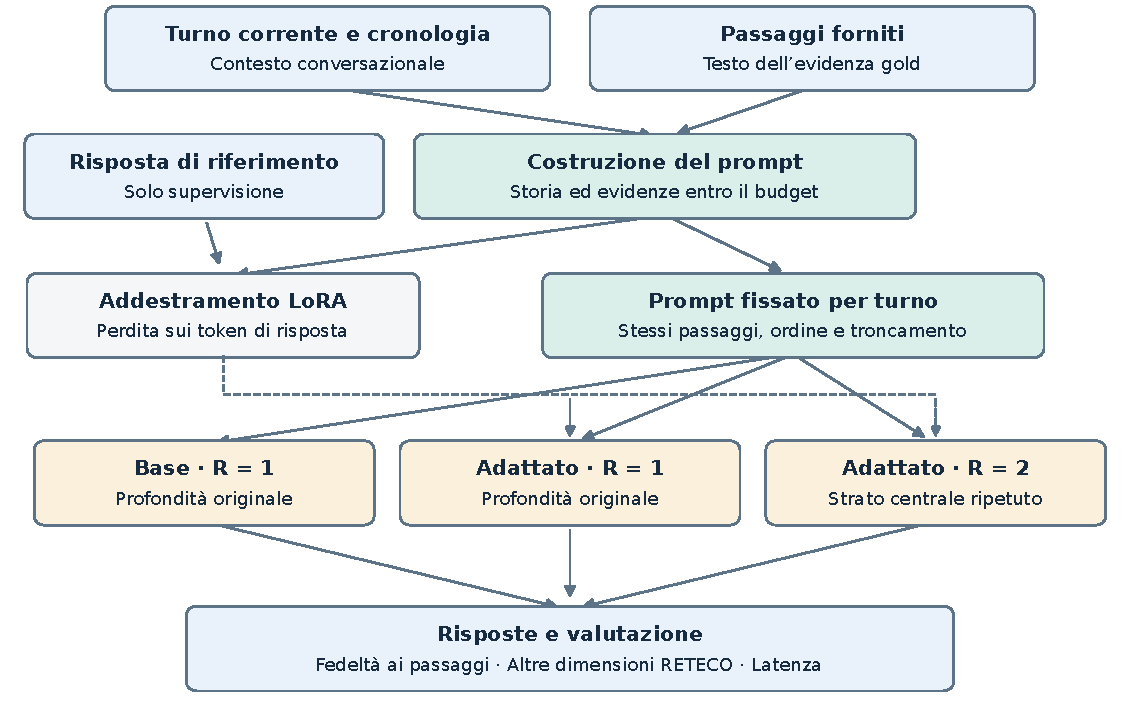
\includegraphics[width=\linewidth]{metodologia_2b.pdf}
 \caption{Flusso del 2b. Il testo dei passaggi forniti dagli organizzatori alimenta il prompt. In addestramento la risposta di riferimento supervisiona i token di uscita. In inferenza lo stesso prompt per turno entra nei bracci a diversa profondità, e le risposte vengono valutate rispetto alle evidenze disponibili. Le frecce tratteggiate indicano il riuso dello stesso adattatore.}
 \label{fig:metodo-2b}
\end{figure}

\paragraph{Adattamento supervisionato.}
Il profilo T4 usa Qwen3-4B-Instruct-2507 con pesi di base quantizzati a 4 bit in formato NF4, calcolo FP16 e adattatori LoRA sulle proiezioni \emph{query} e \emph{value} \cite{lora,qlora}. La configurazione prevede un'epoca, rango 16, $\alpha=32$, dropout 0,05, tasso di apprendimento di riferimento $2\cdot10^{-4}$ e accumulo su otto esempi. L'input di addestramento concatena il prompt $x_t$ alla risposta di riferimento $a_t$. La perdita autoregressiva maschera le posizioni del prompt e del padding:
\begin{equation}
 \ell_t=-\frac{1}{|\mathcal A_t|}\sum_{u\in\mathcal A_t}
 \log p_\theta(a_{t,u}\mid x_t,a_{t,<u}),
 \label{eq:metodo-generazione}
\end{equation}
dove $\mathcal A_t$ contiene le posizioni supervisionate della risposta e $\theta$ indica i parametri del generatore con adattatore. L'equazione esprime la perdita media per un turno, mentre l'implementazione aggrega i token validi del minibatch. In inferenza il prompt termina prima della risposta e il generatore la produce autoregressivamente.

\paragraph{Confronti appaiati.}
Il protocollo prevede tre condizioni sullo stesso insieme di turni: modello base a $R=1$, modello adattato a $R=1$ e stesso modello adattato a $R=2$. Il primo contrasto misura l'effetto dell'adattamento a profondità originale. Il secondo misura l'effetto della profondità a checkpoint fissato. Congeliamo testo, ordine e troncamento dei passaggi, template, cronologia e parametri di generazione. Usiamo decodifica greedy diretta, una risposta per turno, un massimo di 256 nuovi token e penalità di ripetizione 1,05. La fedeltà alle evidenze è la dimensione primaria proposta. Correttezza, completezza, pertinenza e coerenza conversazionale descrivono gli altri aspetti della risposta secondo la rubrica RETECO \cite{evaluation}. Registriamo anche la lunghezza generata e la latenza per risposta, così da interpretare il costo a fronte sia del numero di applicazioni di strato sia del numero di token prodotti.
